\documentclass[a4paper]{article}

%% Language and font encodings
\usepackage[english]{babel}
\usepackage[utf8x]{inputenc}
\usepackage[T1]{fontenc}

%% Sets page size and margins
\usepackage[a4paper,top=3cm,bottom=2cm,left=3cm,right=3cm,marginparwidth=1.75cm]{geometry}

%% Useful packages
\usepackage{amsmath}
\usepackage{graphicx}
\usepackage[colorinlistoftodos]{todonotes}
\usepackage[colorlinks=true, allcolors=blue]{hyperref}

\title{Reporte de Actividad 2\\ Introducción a Jupyter y Phyton}
\author{Michelle Contreras Cossio}
\date{7 de Febrero del 2018}

\begin{document}
\maketitle


\section{Introducción}

En esta actividad nos encontramos por primera vez con la programación, como tal, en Phyton, usando el entorno de programación de Jupyter. A partir de la base de datos del Servicio Meteorológico Nacional, realizamos interpretación y análisis de datos del clima de cierta ciudad, explorando las diferentes herramientas que nos presenta Phyton. 

Phyton es un lenguaje de programación, orientado a objetos, utilizado para aplicaciones o incluso páginas web, además es un lenguaje interpretado, que brinda mayor rapidez en su desarrollo; pandas por su parte, es una librería utilizada para el análisis y estructura de datos. Jupyter Notebook, es el entorno de programación donde estaremos trabajando. 



\section{Actividad Realizada}

Durante la actividad se nos pidió aprender a correr Jupyter Notebook desde una terminal, para poder crear un archivo que alojara el código de esta actividad. Trabajamos con un conjunto de datos, estos fueron obtenidos desde el sitio web del Sistema Meteorológico Nacional, en este caso fue escogida la localidad de Todos Santos, BCS, de la cual obtuvimos un archivo txt con datos climatológicos. 

Nos fue brindado un código, el cual debiamos imitar, pero con nuestros datos, para poder entender algunas funciones básicas de como se manejan los datos en pandas, a continuación se muestra:

\begin{enumerate}
\item En un principio, se cargaron las bibliotecas que utilizamos, estas fueron pandas, numpy y matplotlib, utilizadas para el manejo de datos, números y gráficas, respectivamente.
\item Posteriormente, se leyó el archivo txt creado de datos meteorológicos de Todos Santos y se imprimieron los primeros renglones para verificar que fueran leidos correctamente.
\item Se dio estructura a los datos como un data frame y se verificaron los tipos de categorías con que contabamos. 
\item Combinamos dos columnas que contenian la fecha y hora, dentro de una sola.
\item Con "describe" analizamos aspectos importantes de los datos, como es el promedio por columna, máximos, mínimos, cuartiles, entre otros.
\item Hicimos un filtro o selección de datos, que incluía unicamente los datos con la temperatura dentro del rango entre los 24 y 25 $^{\circ}$ C
\item Calculamos la media, por columnas, de los datos.
\item Empezamos a graficar: 
\begin{itemize}
\item La variación de la rapidez de los vientos, añadiendo título a la gráfica y ejes.
\item La variación de la temperatura y humedad relativa, ambas en una sola gráfica.
\item La variación de la temperatura con respecto al tiempo.
\end{itemize}
\end{enumerate}

Posteriormente, se pidieron seis actividades adicionales:
\begin{enumerate}
\item Crear una gráfica que muestre la rapidez de los vientos y la rapidez de las ráfagas, como funciones del tiempo.
Para esto, se creó un nuevo data frame que incluyera únicamente los datos del 26 de enero del 2018, para poder comparar en un solo día estas rapideces.
\begin{figure}[h!]
  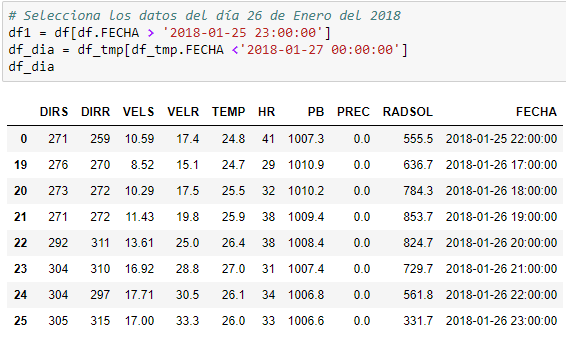
\includegraphics[width=8cm]{1.png}
  \centering
  \label{fig:1}
\end{figure}

Y se graficaron ambas como función de tiempo. Se encontró que las horas del día con más viento son entre la 22 y 23 horas, sin embargo, también se notó que esta hora proporcionada es en UTC, por lo que a la zona horaria que en verdad le corresponde al municipio de Todos Santos, sería a entre 3 y 4 pm. 
\begin{figure}[h!]
  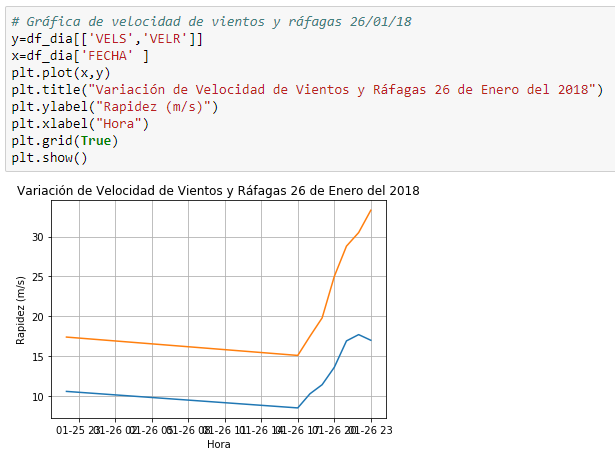
\includegraphics[width=8cm]{2.png}
  \centering
  \label{fig:2}
\end{figure}


\item Crear una gráfica con la dirección de los vientos como función del tiempo. En esta gráfica se utilizaron todos los datos del archivo txt y se encontró que la dirección de los vientos, tipicamente tiene una dirección con un ángulo de entre 260 y 300 grados, los cuales se podrían denominar como los vientos "dominantes" en este caso.

\begin{figure}[h!]
  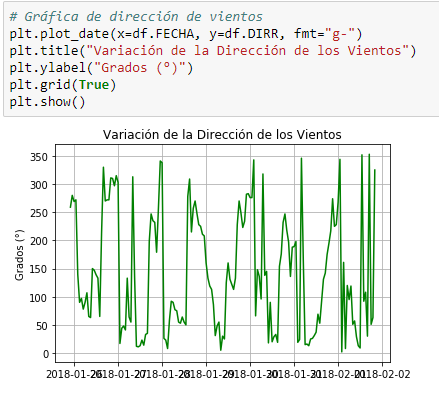
\includegraphics[width=7cm]{3.png}
  \centering
  \label{fig:3}
\end{figure}

\item Muestre el comportamiento de la Radiación Solar como función del tiempo. Se creó, de igual manera, una gráfica que incluyera las fechas, utilizando todos los datos y se encontró que la radiación diariamente y como es de esperar, deciende diariamente hasta cero, y es necesario comentar nuevamente que por la zona horaria que estan manejando, incorrectamente, estos datos, muestra estas ausencias de radiación solar en un rango entre las 2:00 y 13:00 horas, que convertido a horario en Todos Santos, nos da entre las 7:00 pm y 6:00 am, aproximadamente. 

\begin{figure}[h!]
  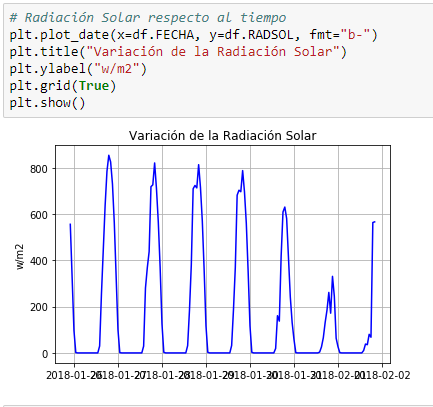
\includegraphics[width=8cm]{4.png}
  \centering
  \label{fig:4}
\end{figure}

También podemos notar que por algunos días, el máximo diario de radiación solar comenzó a decscender y este se ubica, aproximadamente, a las 12:00 horas.

\item ¿Cuál es el lapso de temperatura diaria? Para responder esta pregunta, se creó, nuevamente, una gráfica de la variación de la temperatura, con respecto al 26 de enero del 2018 y para calcular el rango de variación de la temperatura, se restó la Temperatura máxima menos la mínima. Esto nos dió un total de 2.3$^{\circ}$ C.

\begin{figure}[h!]
  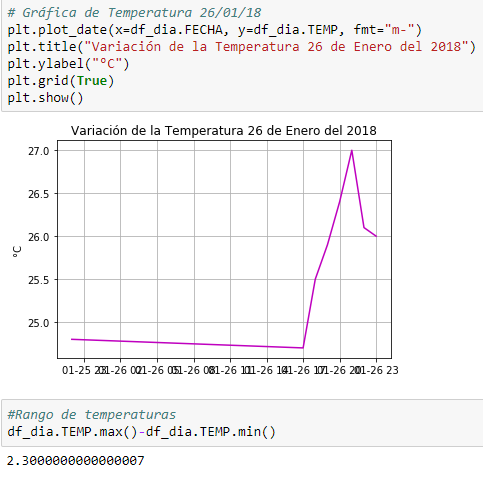
\includegraphics[width=8cm]{5.png}
  \centering
  \label{fig:5}
\end{figure}

\item ¿Puedes comentar sobre la relación entre la temperatura y la humedad relativa? Para ello se utilizó la gráfica creada mediante el uso del ejemplo. 

En la gráfica no pude notar ningún patron de dependencia entre estas dos variables, en ciertos puntos tienen picos al mismo tiempo, pero en otros momentos, mientras la temperatura disminuye, la humedad relativa aumenta.

\begin{figure}[h!]
  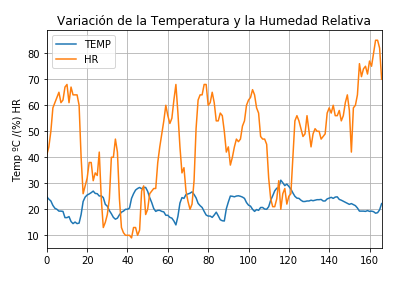
\includegraphics[width=8cm]{6.png}
  \centering
  \label{fig:6}
\end{figure}

\item Realiza el análisis exploratorio de datos, que resuma el sitio estudiado, se realizó el describe sobre los datos que contienen a todo el archivo txt: 

\begin{figure}[h!]
  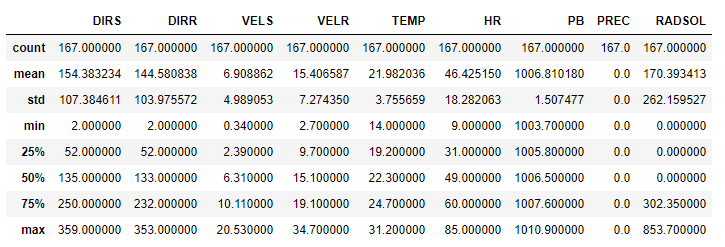
\includegraphics[width=14cm]{7.png}
  \centering
  \label{fig:7}
\end{figure}

\end{enumerate}


\section {Investigación}
En esta sección se añade la información extra, recabada de internet, para el mayor y mejor entendimiento de las funciones y características de la biblioteca y entorno utilizados. 


\subsection{Jupyter}

Como fue mencionado con anterioridad, Jupyter Notebook es un ambiente de programación que permite editar código, widgets, texto, ecuaciones, imagenes, video, los cuales se pueden convertir a diferentes formatos y compartir facilmente. 

\subsubsection{Características}
Jupyter Notebook contiene tres componentes principales: 
\begin{itemize}
\item Aplicación web: su aplicación interactiva, donde se puede editar y crear código y documentos "notebook". Esta edita y corre código, permite crear widgets de JavaScript e incluye ecuaciones matemática.
\item Kernels: son procesos separados que corren el código del usuario, en cierto lenguaje, en la aplicación web y muestran la salida directamente en la aplicación. Cuenta con kernels que soportan: Phyton, R, Julia, Ruby, Haskell, Scala, node.js, Go.
\item Documentos "notebook": documentos que contienen una representación de lo que se ve en la aplicación web, todas las entradas y salidas, imagenes, ecuaciones, etc. Cada notebook tiene su propio kernel. Los notebooks consisten en una sucesión de celdas y tienen la extensión ".ipynb", pero pueden exportarse en diferentes formatos como PDF o LaTeX.
\end{itemize}

\subsubsection{Ventajas}
\begin{itemize}
\item Se puede usar en prácticamente cualquier lugar, es un software libre disponible en diferentes sistemas operativos y fácil de instalar. 
\item Soporta una amplia variedad de lenguajes de programación, entre los que destaca Phyton, R, Ruby, entre otros.
\item Es interactivo, te brinda inmediatamente el "feedback" o salida del código.
\item Es open source, permite a los usuarios revisarlo y proponer cambios o extensiones, incluso es posible personalizarlo para un uso específico.
\item Produce gráficas, tablas entre otras capacidades matemáticas, es muy utilizado en la ciencia.
\end{itemize}

\subsubsection{Desventajas}
\begin{itemize}
\item Aunque es útil que sea interactivo, es un poco difícil acostumbrarse a esto.
\item Es más complicado instalarlo y acomodarlo todo para un primer uso, que otros entornos de programación. 
\item No es fácil configurarlo para poder compartirlo y editar en otra computadora, es necesario realizar ciertos pasos que no podrían resultar triviales para cualquier usuario.
\item Es dificil poder trabajar de manera colaborativa con este entorno, por lo mismo que no es sencillo "abrir" el código en otra computadora, como se revisó en el punto anterior.
\end{itemize}


\subsection{Phyton: Pandas}

Pandas es un paquete de Phyton que facilita el trabajar con datos. 

Provee estructuras de datos de manera rápida y flexible y promete ser el analista y manipulador de datos, en open source, más poderoso, disponible en cualquier lenguaje. 

Trabaja muy bien en el manejo de varios tipos de datos, ya sean tabulares, datos observacionales o estadísticos, entre otros.

\subsubsection{Ventajas}
\begin{itemize}
\item Reporta cuando se tienen datos perdidos.
\item Permite el cambio de tamaño de los datos, se pueden intertar o eliminar columnas del data frame.
\item Buenas herramientas IO que permiten cargar datos desde archivos planos, bases de datos, archivos excel y guardarlos en un formato HDf5 ultra rápido. 
\item Pandas es rápido.
\item Se usa en la producción de aplicaciones financieras.
\item Permite un manejo de bases de datos bastante extensas.
\item Es fácil de usar y fácil de aprender.
\end{itemize}

\subsubsection{Desventajas}
\begin{itemize}
\item Cuenta con mucha competencia, como es excel, con el que es bastante comparado, ya que también permite el uso de bases de datos, de una manera un poco más sencilla para un usuario inexperimentado en el uso de código. 
\end{itemize}

\subsubsection{Herramientas útiles}
A continuación se presentan algunas funciones básicas que pueden parecer útiles al momento de trabajar con pandas:
\begin{itemize}

\item Para análisis o inspección de datos: 
\begin{itemize}
\item df.mean(), muestra el promedio de todas las columnas.
\item df.corr(), muestra la correlación entre columnas.
\item df.count(), muestra el número de datos.
\item df.max(), muestra el máximo de cada columna.
\item df.min(), muestra el mínimo de cada columna.
\item df.median(), muestra la mediana de cada columna.
\item df.std(), muestra la desviación estándar de cada columna.
\end{itemize}

\item Para selección de datos:
\begin{itemize}
\item (df[col]), selecciona una columna como un nuevo data frame.
\item (df[[col1, col2]]), selecciona dos columnas como un nuevo data frame.
\item (s.iloc[0]), selecciona por posición.
\end{itemize}

\item Para el filtro de datos: 
\begin{itemize}
\item df[df[year] > 1984], brindará las columnas donde el año es mayor que 1984.
\item df.groupby(col), separa, según un criterio específico, en grupos, aplica una función a cada grupo, de manera independiente y combina el resultado en una estructura de datos. 
\end{itemize}

\end{itemize}


\section{Apéndice}
\begin{enumerate}
\item ¿Cuál es tu primera impresión de Jupyter Notebook?

Al principio no entendía de que se trataba, ya que el entorno donde estaba acostumbrada a trabajar era en una aplicación descargada en la computadora (Geany), estaba acostumbrada a trabajar con el lenguaje Fortran, que es un lenguaje compilado; por otro lado, en Phyton no es necesario compilar y eso me resultó más fácil.

\item ¿Se te dificultó leer código en Python?

Si, pero con los letreros que presentó el maestro he ido entendiendo, aunque no del todo, entiendo la estructura, pero no algunas banderas u opciones que se presentan. 

\item ¿En base a tu experiencia de programación en Fortran, que te parece el entorno de trabajar en Python?

Mucho más sencillo ya que la estructura y sintaxis es menos complicada, sin embargo, como ya mencione, hay muchos comandos que aun no entiendo. 

\item A diferencia de Fortran, ahora se producen las gráficas utilizando la biblioteca Matplotlib. ¿Cómo fue tu experiencia?. 

Lás gráficas son visualmente más atractivas y fáciles de producir que con Gnuplot, Phyton es un lenguaje con mejor estética que Fortran y eso me agrada.

\item En general, ¿qué te pereció el entorno de trabajo en Python? 

Por lo pronto, es sencillo de usar, fácil de instalar en cualquier computadora con cualquier SO. 

\item ¿Qué opinas de la actividad? ¿Estuvo compleja? ¿Mucho material nuevo? ¿Que le faltó o que le sobró? ¿Qué modificarías para mejorar? 

Me gustó la actividad como iniciación a Phyton, no fue compleja pero si es un poco difícil encontrar resultados web de cierto problema, ya que Phyton es un lenguaje bastante recurrido y hay demasiada información, que en cierto punto es difícil de digerir. Si fue mucho material nuevo, pero el suficiente. 

\item ¿Comentarios adicionales que desees compartir? 

Phyton, hasta este punto, me esta gustando, pero tengo que leer mucho de las funciones que ofrece, para poder entender mejor cuando busque soluciones, en foros, por ejemplo.
\end{enumerate}


\section{Referencias Bibliográficas}
\begin{itemize}
\item https://desarrolloweb.com/articulos/1325.php
\item https://jupyter-notebook.readthedocs.io/en/stable/examples/Notebook/What\%20is\%20the\\
\%20Jupyter\%20Notebook.html
\item https://www.quora.com/What-are-the-pros-and-cons-of-using-Python-Jupyter-versus-a-normal-Python-development-environment 
\item https://www.slant.co/topics/366/viewpoints/23/~best-python-ides~jupyter
\item https://www.dataquest.io/blog/jupyter-notebook-tips-tricks-shortcuts/
\item https://pandas.pydata.org/pandas-docs/stable/index.html
\item https://towardsdatascience.com/a-quick-introduction-to-the-pandas-python-library-f1b678f34673
\end{itemize}

%
\end{document}